\documentclass{standalone}
\usepackage{tikz}
\usepackage{tikz-qtree}
\usepackage[makeroom]{cancel}
\usetikzlibrary{fit}


\begin{document} 
	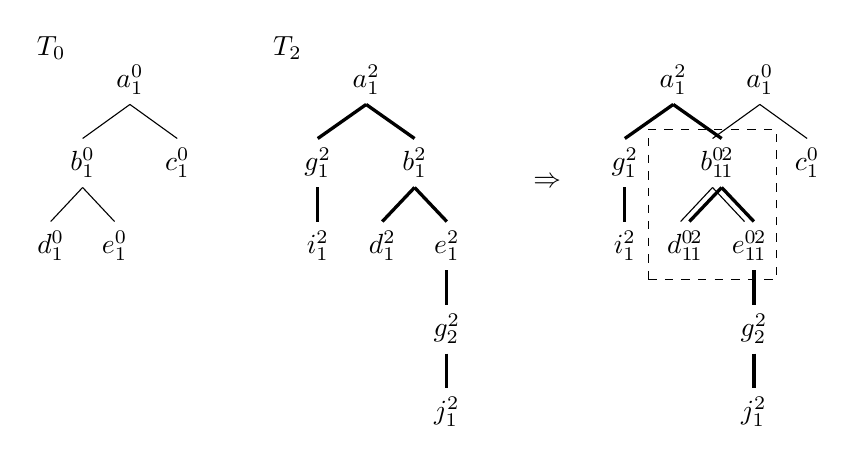
\begin{tikzpicture}[sibling distance=7pt]
	\tikzset{level 1+/.style={level distance=2.5\baselineskip}}

	    \node (x) at (-1,0.5) {$T_0$} ;
	    \Tree [.$a_1^0$
	            [.$b_1^0$
	                [.$d_1^0$ ]
	                [.$e_1^0$ ] 
	            ] 
	            [.$c_1^0$ ]
	          ]
	    

	    \begin{scope}[xshift=3.0cm]
	    \tikzset{edge from parent/.style={very thick,draw}}
	    \node (y) at (-1,0.5) {$T_2$} ;
	    \Tree [.$a_1^2$
	            [.$g_1^2$
	                [.$i_1^2$ ]
	            ]  
	            [.$b_1^2$
	            	[.$d_1^2$ ]
	            	[.$e_1^2$ 
	            		[.$g_2^2$ 
	            			[.$j_1^2$ ]
	            		]
	            	]
	            ]
	          ]
		\node (arrow1) at (2.3,-1.2) {$\Rightarrow$};
	    \end{scope}



	    \begin{scope}[xshift=8.0cm]
	    \Tree [.$a_1^0$
	            [.\node(b){$b_1^0$};
	                [.\node(d){$d_1^0$}; ]
	                [.\node(e){$e_1^0$}; ] 
	            ] 
	            [.\node(c){$c_1^0$}; ]
	          ]
	    
	    \node[draw,dashed,fit=(b)(d)(e)]{};
	    \end{scope}



		\begin{scope}[xshift=6.9cm]
		\tikzset{edge from parent/.style={very thick,draw}}
	    \Tree [.$a_1^2$
	            [.$g_1^2$
	                [.$i_1^2$ ]
	            ]  
	            [.$\phantom{b}_1^2$
	            	[.$\phantom{d}_1^2$ ]
	            	[.$\phantom{e}_1^2$ 
	            		[.$g_2^2$ 
	            			[.$j_1^2$ ]
	            		]
	            	]
	            ]
	          ]
		\end{scope}


	\end{tikzpicture}
\end{document} 